\documentclass[journal,transmag]{IEEEtran}

\usepackage{lipsum}
\usepackage{graphicx}
\usepackage{float}
\usepackage{booktabs} % For better table formatting
\usepackage{caption}  % For caption formatting
%\usepackage{cite}


% *** GRAPHICS RELATED PACKAGES ***
%
\ifCLASSINFOpdf
\else
\fi
\usepackage[cmex10]{amsmath}

\begin{document}

\title{Black-Litterman Portfolio\\ Optimization with Linear Algebra in Python}

\author{
    \IEEEauthorblockN{Otto, Tom, Ada}
}
\IEEEtitleabstractindextext{%
\begin{abstract}
This paper presents a comprehensive implementation of the Black-Litterman portfolio optimization model using Python
and linear algebra techniques. We combine traditional Markowitz mean-variance optimization with sentiment analysis of financial news 
to generate market views. The implementation leverages historical price data and news sentiment scores to construct optimal 
portfolio weights. Our results demonstrate how incorporating news sentiment as a source of market views can enhance the classical Black-Litterman framework.
We provide a detailed mathematical foundation of the model and discuss practical considerations for implementation. 
The complete code implementation and analysis are made available through a public repository.

\end{abstract}
}

\maketitle


\IEEEdisplaynontitleabstractindextext
\IEEEpeerreviewmaketitle



\section{Introduction}
When deciding on how to allocate a portfolio in the stock market, two of the most important factors are risk and return. Typically risk or volatility is 
measured by the variance of a stock. The problem becomes that many high-return stocks or assets also have high variance. In 1959, Harry Markowitz 
introduced a model that would allow for the optimization of a portfolio by balancing risk and return. This model is known as the Markowitz model \cite{markowitz1959} and 
it has become the basis for modern portfolio theory. 

In our following paper, we will be implementing the Black-Litterman model \cite{black1992global} which is a modification of the Markowitz model using 3 risky assets. 
\section{Markowitz Model}
We begin by optiaining the daily closing prices of GOOGL, AAPL, and AMZN from 2020-2024 and calculate the log returns. We use 
log returns because they are additive and easier to work with. 

\begin{equation}
\text{Log Returns} = \ln\left(\frac{P_t}{P_{t-1}}\right)
\end{equation}

We define a portfolio as $X$ such that:
\begin{equation}
x_A + x_B + x_C = 1
\end{equation}

\noindent Meaning that the sum of the percentage of the portfolio in each asset must equal 100\%. The return of the portfolio is the following:

\begin{equation}
\mu_{p,x} = E[R_{p,x}] = x_A \mu_A + x_B \mu_B + x_C \mu_C
\end{equation}

\noindent We find the expected return of each asset by taking the mean of the log returns. We find the covariance matrix by taking the covariance of the log returns.
\begin{equation}
E[\mathbf{R}] = E \left[ \begin{pmatrix} R_A \\ R_B \\ R_C \end{pmatrix} \right] = \begin{pmatrix} E[R_A] \\ E[R_B] \\ E[R_C] \end{pmatrix} = \begin{pmatrix} \mu_A \\ \mu_B \\ \mu_C \end{pmatrix}
\end{equation}

\begin{equation}
\Sigma = \begin{pmatrix} \sigma_A^2 & \sigma_{AB} & \sigma_{AC} \\ \sigma_{BA} & \sigma_B^2 & \sigma_{BC} \\ \sigma_{CA} & \sigma_{CB} & \sigma_C^2 \end{pmatrix}
\end{equation}

\noindent To obtain the variance and standard deviation of the portfolio,
we take the matrix multiplication of the portfolio weights and the covariance matrix and then the square root for the standard deviation.

\begin{equation}
\sigma_{p,x}^2 = \mathbf{w}^T \Sigma \mathbf{w}
\end{equation}

\begin{equation}
\sigma_{p,x} = \sqrt{\sigma_{p,x}^2}
\end{equation}

\noindent And we take the matrix multiplication of the weights and the expected returns to find the return of the portfolio.

\begin{equation}
\mu_{p,x} = \mathbf{w}^T \mu
\end{equation}

To confirm our later results, we plot the standard deviation vs the expected return using 10,000 random points.

\begin{figure}[H]
\centering
\includegraphics[width=0.45\textwidth]{assets/standard_deviation_vs_expected_return.png}
\caption{Standard Deviation vs Expected Return}
\end{figure}

\section{Global Minimum Variance Portfolio}
We must find the minimum variance portfolio given the constraints:

\begin{equation}
\text{min} ~ \sigma_{p,x}^2 = \mathbf{w}^T \Sigma \mathbf{w}
\end{equation}

\noindent Such that
\begin{equation}
m_A + m_B + m_C = 1
\end{equation}

If our goal is to minimize the variance, we can use the langrangian to to optimize the portfolio given a constraint. 
If we remember, the langrangian multiplier is defined as $\nabla f = \lambda \nabla g, \quad g = 0$ 
where $f$ is the objective function and $g$ is the constraint. 

\begin{equation}
\mathcal{L} = \sigma_{p,x}^2 + \lambda (m_A + m_B + m_C - 1)
\end{equation}

\noindent Taking the partial derivatives we get 


\begin{align}
\frac{\partial \mathcal{L}}{\partial w_A} &= 2w_A\sigma_A^2 + 2w_B\sigma_{AB} + 2w_C\sigma_{AC} + \lambda = 0 \\
\frac{\partial \mathcal{L}}{\partial w_B} &= 2w_B\sigma_B^2 + 2w_A\sigma_{AB} + 2w_C\sigma_{BC} + \lambda = 0 \\
\frac{\partial \mathcal{L}}{\partial w_C} &= 2w_C\sigma_C^2 + 2w_A\sigma_{AC} + 2w_B\sigma_{BC} + \lambda = 0 \\
\frac{\partial \mathcal{L}}{\partial \lambda} &= w_A + w_B + w_C - 1 = 0
\end{align}


\noindent This gives us a system of linear equations that can be written in matrix form:

\begin{equation}
\begin{bmatrix} 
2\sigma_A^2 & 2\sigma_{AB} & 2\sigma_{AC} & 1 \\
2\sigma_{AB} & 2\sigma_B^2 & 2\sigma_{BC} & 1 \\
2\sigma_{AC} & 2\sigma_{BC} & 2\sigma_C^2 & 1 \\
1 & 1 & 1 & 0
\end{bmatrix}
\begin{bmatrix}
w_A \\
w_B \\
w_C \\
\lambda
\end{bmatrix} = 
\begin{bmatrix}
0 \\
0 \\
0 \\
1
\end{bmatrix}
\end{equation}

Plotting this against the random points we get the following:
\begin{figure}[H]
\centering
\includegraphics[width=0.4\textwidth]{assets/global_minimum_variance_portfolio.png}
\caption{Global Minimum Variance Portfolio}
\end{figure}

\section{Efficient Frontier}
One consequence of the Markowitz model is the efficient frontier, the set of portfolios that offer the maximum return for a given level of risk,
or minimum risk for a given level of return. In the next equations, we will be optimizing the efficient frontier of a function of the return. 


\begin{equation}
  \text{min } \sigma_p^2 = \mathbf{x}' \Sigma \mathbf{x}
\end{equation}

Subject to two constrainst:
\begin{equation}
  \mathbf{x}' \mu = \mu_p \text{ (target return)}
\end{equation}

\begin{equation}
x'1 = 1 \text{ (weights sum to 1)}
\end{equation}

\noindent We can use the langrangian once again to optimize, but this time we have two constraints. 

\begin{equation}
  \mathcal{L}(x, \lambda_1, \lambda_2) = \mathbf{x}' \Sigma \mathbf{x} + \lambda_1 (\mathbf{x}' \mu - \mu_p) + \lambda_2 (1 - \mathbf{x}' 1)
\end{equation}

\noindent Taking the partial derivatives we get:

\begin{align}
\frac{\partial \mathcal{L}(x, \lambda_1, \lambda_2)}{\partial \mathbf{x}} &= 2\Sigma \mathbf{x} + \lambda_1 \mu + \lambda_2 \mathbf{1} = 0, \\
\frac{\partial \mathcal{L}(x, \lambda_1, \lambda_2)}{\partial \lambda_1} &= \mathbf{x}' \mu - \mu_p = 0, \\
\frac{\partial \mathcal{L}(x, \lambda_1, \lambda_2)}{\partial \lambda_2} &= \mathbf{x}' \mathbf{1} - 1 = 0.
\end{align}



We are then given a linear system, which we are able to solve:

\begin{equation}
\begin{bmatrix} 
2\Sigma & \mathbf{\mu} & \mathbf{1} \\
\mathbf{\mu}' & 0 & 0 \\
\mathbf{1}' & 0 & 0
\end{bmatrix}
\begin{bmatrix}
\mathbf{x} \\
\lambda_1 \\
\lambda_2
\end{bmatrix} = 
\begin{bmatrix}
0 \\
\mu_p \\
1
\end{bmatrix}
\end{equation}

It can be shown that all portfolios on the efficient frontier are linear combinations of any two minimum variance portfolios \cite{zivot2013}.

Let $\alpha$ be any constant and define the portfolio $\mathbf{z}$ as a linear combination of portfolios $\mathbf{x}$ and $\mathbf{y}$:

\begin{equation}
\mathbf{z} = \alpha \cdot \mathbf{x} + (1 - \alpha) \cdot \mathbf{y}
\end{equation}

which results in:

\begin{equation}
\mathbf{z} = 
\begin{pmatrix}
\alpha x_A + (1 - \alpha) y_A \\
\alpha x_B + (1 - \alpha) y_B \\
\alpha x_C + (1 - \alpha) y_C
\end{pmatrix}
\end{equation}

By picking any two optimal portfolios and plotting the for different linear combinations $\alpha = (0,1)$ we get this for the efficient frontier:
\begin{figure}[H]
  \centering
  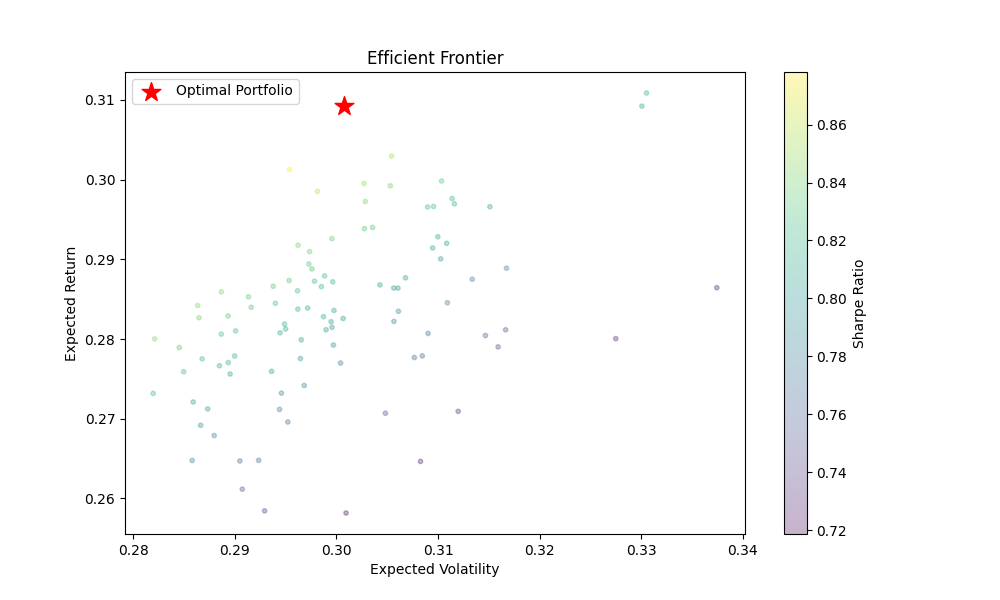
\includegraphics[width=0.45\textwidth]{assets/efficient_frontier.png}
  \caption{Efficient Frontier}
  \end{figure}
\section{Sharpe Ratio}
The Sharpe Ratio is a measure used to evaluate the risk-adjusted return of an investment portfolio.
It is calculated by subtracting the risk-free rate from the portfolio's return and then dividing the 
result by the portfolio's standard deviation. Mathematically, it is expressed as:

\begin{equation}
\text{Sharpe Ratio} = \frac{R_p - R_f}{\sigma_p}
\end{equation}

where \( R_p \) is the return of the portfolio, \( R_f \) is the risk-free rate, and \( \sigma_p \) is the standard deviation of the portfolio's returns. A higher Sharpe Ratio indicates a more attractive risk-adjusted return. To finish off the analysis, we can calculate the Sharpe Ratio for the optimal portfolios.

After lengthly calculations \cite{zivot2013}, optimizing said ratio, it can be shown that it can be computed as:

\begin{equation}
\mathbf{t} = \frac{\Sigma^{-1}(\boldsymbol{\mu} - r_f \cdot \mathbf{1})}{\mathbf{1}'\Sigma^{-1}(\boldsymbol{\mu} - r_f \cdot \mathbf{1})}
\end{equation}

\noindent where $\mathbf{t}$ is the tangency portfolio. 

\begin{figure}[H]
  \centering
  \includegraphics[width=0.45\textwidth]{assets/tangency_portfolio.png}
  \caption{Tangency Portfolio}
  \end{figure}

\section{Conclusion}
\lipsum[1]

\ifCLASSOPTIONcaptionsoff
  \newpage
\fi


\begin{thebibliography}{1}
%Insert any references here
\bibitem{zivot2013}
E.~Zivot, ``Portfolio Theory with Matrix Algebra,'' \emph{University of Washington}, 2013.
\bibitem{black1992global}
F.~Black and R.~Litterman, ``Global Portfolio Optimization,'' \emph{Financial Analysts Journal}, vol.~48, no.~5, pp.~28--43, 1992.
\bibitem{markowitz1959}
Markowitz, H. (1959). Portfolio Selection: Efficient Diversification of Investments, Wiley, New York.
\end{thebibliography}


\end{document}